% ========================================================
% Introduction 

\minitoc

L'informatique graphique est une discipline définissant différents modèles et algorithmes pour modéliser numériquement des scènes et des objets. Pour cela, elle se base sur des notions de Mathématiques Appliquées, Géométrie Différentielle et d'Optimisation. 
L'ojectif est de proposer à des graphistes, des dessinateurs, ou des ingénieurs des algorithmes et logiciels capables de modéliser et visualiser tout types de formes, d'un personnage d'animation à une pièce à usiner. 

Historiquement, l'informatique graphique se regroupe sur trois sous-disciplines transverses. La première se concentre sur \emph{l'animation} : on cherche ici à développer des modèles pour animer des pièces déjà créées. Par exemple on peut chercher à définir des rotations à appliquer à des objets pour décrire le mouvement d'un personnage. 
La seconde est le \emph{rendu en temps réel}. On cherche ici à donner de la texture à une animation en temps réel pour donner à un utilisateur une vision acceptable de sa scène. Par exemple, on peut s'intéresser au rendu temps réel dans un jeu vidéo où l'utilisateur doit avoir sous les yeux des images qui rentrent dans la charte graphique de son jeu tout en gardant une fluidité suffisante d'affichage à l'écran. 
Enfin, le \emph{rendu physiquement réaliste} cherche à rendre une image ou une scène la plus réaliste possible. Ici, on cherchera à simuler au plus près les jeux de lumière sur la matière pour donner une vision la plus réaliste possible à l'utilisateur. 

L'objectif de ce cours et de proposer des méthodes mathématiques et algorithmiques permettant la création et la modélisation d'environnements en 3D et le traitement d'une géométrie à partir d'une capture. 

% ======================================================================
% Section 1 : Cadre mathématique et prérequis géométriques

\section{Cadre mathématique et prérequis géométriques}

La modélisation géométrique vise à représenter et manipuler des formes numériques par des outils d'analyse et d'algèbre linéaire. Contrairement à une description discrète (maillages polygonaux), on privilégie ici une modélisation paramétrique continue à haut niveau.

Pour construire cette modélisation paramétrique, nous nous basons sur des \emph{points de contrôles}. Ces points seront définis par l'utilisateur et serviront de base pour générer une \emph{courbe approximante} de la forme qu'ils décrivent. 

% ----------------------------------------------------------------------
\subsection{Espaces affines et arithmétique des points}

En synthèse d'images et en modélisation, il est donc fondamental de distinguer les notions d'\emph{emplacements} (points) et de \emph{déplacements} (vecteurs). Pour les premiers, nous utilisons la notions \emph{d'espace affine} pour les définir formellement. 

\begin{definition}[Espace affine]
    Soit $E$ un $\R$-espace vectoriel. Un \emph{espace affine} attaché à $E$ est un ensemble non vide $\mathcal{E}$ muni d'une action libre et transitive du groupe additif $(E, +)$ sur $\mathcal{E}$ :
    \begin{equation}
        \begin{aligned}
            \Phi : \mathcal{E} \times E &\longrightarrow \mathcal{E} \\
            (A, \vec{v}) &\longmapsto A + \vec{v}
        \end{aligned}
    \end{equation}
    qui vérifie :
    \begin{enumerate}
        \item $\forall A \in \mathcal{E}, \; A + \vec{0} = A$ ;
        \item $\forall A \in \mathcal{E}, \; \forall \vec{u}, \vec{v} \in E, \; (A + \vec{u}) + \vec{v} = A + (\vec{u} + \vec{v})$ ;
        \item $\forall A, B \in \mathcal{E}$, il existe un unique vecteur noté $\vec{AB} \in E$ tel que $B = A + \vec{AB}$.
    \end{enumerate}
    La dimension de $\mathcal{E}$ est par définition la dimension de $E$. Dans la suite, on considérera $\mathcal{E} \simeq \R^2$ ou $\R^3$.
\end{definition}

On définira donc l'espace des points comme un \emph{espace affine} dans lequel nous ne pourrons effectuer que ces opérations. À noter que les opérations sur les points ainsi que leur définition sont \emph{indépendantes} du repère utilisé. 

\begin{remark}[Opérations licites]
    L'espace affine n'est pas muni d'une addition interne naturelle sur ses éléments. Ainsi :
    \begin{itemize}
        \item La somme de deux points $A + B$ n'a \emph{aucun sens géométrique} intrinsèque (elle dépendrait de l'origine choisie).
        \item La différence de deux points $B - A$ est un vecteur bien défini ($\vec{AB} \in E$).
        \item La translation d'un point par un vecteur $A + \vec{v}$ est un point bien défini de $\mathcal{E}$.
    \end{itemize}
\end{remark}

% ----------------------------------------------------------------------
\subsection{Combinaisons affines et barycentres}

Pour interpoler ou moyenner des positions de points de contrôle, nous avons besoin d'une opération linéaire adaptée à l'espace affine.

\begin{definition}[Combinaison affine et Barycentre]
    Soit $(P_0, \dots, P_n) \in \mathcal{E}^{n+1}$ une famille finie de points et $(\alpha_0, \dots, \alpha_n) \in \R^{n+1}$ une famille de scalaires.
    
    L'expression formelle $\sum_{i=0}^n \alpha_i P_i$ n'est indépendante de tout repère d'origine $O \in \mathcal{E}$ si et seulement si la somme des poids vérifie la \emph{condition de partition de l'unité} :
    \begin{equation}
        \sum_{i=0}^n \alpha_i = 1
    \end{equation}
    Dans ce cas, le point $G \in \mathcal{E}$ défini de manière unique par :
    \begin{equation}
        \sum_{i=0}^n \alpha_i \vec{GP_i} = \vec{0} \iff G = O + \sum_{i=0}^n \alpha_i \vec{OP_i} \quad (\forall O \in \mathcal{E})
    \end{equation}
    est appelé le \emph{barycentre} du système pondéré $\{(P_i, \alpha_i)\}_{i=0}^n$, noté par abus $G = \sum_{i=0}^n \alpha_i P_i$.
\end{definition}

\begin{definition}[Enveloppe convexe]
    Une combinaison affine est dite \emph{convexe} si de plus tous les coefficients sont positifs ou nuls :
    \begin{equation}
        \forall i \in \llbracket 0, n \rrbracket, \; \alpha_i \geqslant 0 \quad \text{avec} \quad \sum_{i=0}^n \alpha_i = 1
    \end{equation}
    L'\emph{enveloppe convexe} d'un ensemble de points $\mathcal{P} = \{P_0, \dots, P_n\}$, notée $\mathrm{Conv}(\mathcal{P})$, est l'ensemble de toutes leurs combinaisons convexes :
    \begin{equation}
        \boxed{\mathrm{Conv}(\mathcal{P}) := \left\{ \sum_{i=0}^n \alpha_i P_i \;\middle|\; \alpha_i \geqslant 0, \; \sum_{i=0}^n \alpha_i = 1 \right\}}
    \end{equation}
\end{definition}

En topologie affine, $\mathrm{Conv}(\mathcal{P})$ correspond au plus petit ensemble convexe fermé contenant $\mathcal{P}$. C'est une propriété stabilisatrice clé : toute courbe construite par mélange convexe reste confinée dans cette zone sans divergence numérique.

% ----------------------------------------------------------------------
\subsection{Courbes paramétrées}

Une fois nos \emph{points de contrôles} définis, nous allons définir une courbe approximante de ces points. Nous utilisons pour cela les \emph{courbes paramtriques}. 

\begin{definition}[Courbe paramétrée]
    Une \emph{courbe paramétrée} $C$ dans $\mathcal{E}$ de classe $ \mathcal{C}^k$ est la donnée d'une application $f : I \subset \R \longrightarrow \mathcal{E}$ de classe $ \mathcal{C}^k$. 
    On posera $I = [u_{\min}, u_{\max}]$ un intervalle fermé de $\R$. On posera donc : 
    \begin{equation}
        C = f(I) = \{f(u) \mid u \in I\} \subset \mathcal{E}. 
    \end{equation}
\end{definition}

% En informatique graphique, il est capital de découpler le comportement analytique de la paramétrisation choisie de la forme intrinsèque de la courbe tracée à l'écran.

% \begin{definition}[Continuité paramétrique $C^k$ vs géométrique $G^k$]
%     Soient deux arcs de courbes réguliers $P_1 : [a, b] \to \mathcal{E}$ et $P_2 : [b, c] \to \mathcal{E}$ se raccordant en $P_1(b) = P_2(b)$ :
%     \begin{itemize}
%         \item \textbf{Continuité paramétrique $C^k$} : Les $k$ premières dérivées vectorielles coïncident au raccord :
%         \begin{equation}
%             \forall j \in \llbracket 0, k \rrbracket, \quad \frac{d^j P_1}{d u^j}(b^-) = \frac{d^j P_2}{d u^j}(b^+)
%         \end{equation}
%         Elle dépend explicitement de la vitesse de parcours du paramètre $u$.
%         \item \textbf{Continuité géométrique $G^k$} : Il existe un reparamétrage régulier $\varphi$ admissible tel que la courbe résultante soit de classe $C^k$. En particulier :
%         \begin{itemize}
%             \item $G^0 \iff C^0$ : continuité simple des positions ($P_1(b) = P_2(b)$) ;
%             \item $G^1$ : les vecteurs tangents ont même direction et même sens, à un facteur d'échelle strictement positif près :
%             \begin{equation}
%                 \exists \lambda > 0, \quad P_2'(b^+) = \lambda \, P_1'(b^-)
%             \end{equation}
%             \item $G^2$ : continuité des centres et rayons de courbure aux points de raccordement, garantissant une absence de rupture visuelle d'inflexion.
%         \end{itemize}
%     \end{itemize}
% \end{definition}


% ======================================================================
% Section 2 : Représentations polynomiales

\section{Représentations polynomiales}

L'objectif est de modéliser des courbes ou des surfaces par des représentations paramétriques continues. Contrairement aux maillages discrets, cette approche dite de \emph{haut niveau} offre une empreinte mémoire réduite et garantit un tracé parfaitement lisse.

Pour manipuler ces formes, on introduit une famille de \emph{points de contrôle} $(P_0, \dots, P_n)$. Ces points servent d'interface intuitive à l'utilisateur pour contraindre la géométrie globale. Idéalement, la courbe générée doit satisfaire trois propriétés géométriques fondamentales :
\begin{enumerate}
    \item \textbf{Diminution de la variation :} la courbe ne doit pas osciller davantage que son polygone de contrôle.
    \item \textbf{Confinement convexe :} la courbe doit être entièrement contenue dans l'enveloppe convexe formée par ses points de contrôle.
    \item \textbf{Invariance par symétrie :} le tracé ne doit pas dépendre du sens de parcours des indices des points.
\end{enumerate}

% ----------------------------------------------------------------------
\subsection{Interpolation vs Approximation}

La première approche, naturelle, consiste à chercher une courbe qui \emph{interpole} strictement tous les points de contrôle. Cependant, l'interpolation polynomiale globale (comme celle de Lagrange) devient rapidement instable à mesure que le nombre de points augmente. Comme l'illustre la Figure~\ref{fig:lagrange_runge} avec le phénomène de Runge, le polynôme produit de fortes oscillations parasites aux extrémités et s'échappe largement de l'enveloppe convexe des données.

\begin{figure}[htbp]
    \centering
    -- Ajouter figure --
    \caption{}
    \label{fig:lagrange_runge}
    % TODO : Ajouter figure interpolation de Lagrange. 
\end{figure}

Face à ces limites, on privilégie l'approche par \emph{approximation}. Plutôt que d'imposer le passage par chaque point intermédiaire, on utilise les points de contrôle comme des "attracteurs". On garantit ainsi le lissage, la stabilité numérique et le respect strict des contraintes géométriques énoncées ci-dessus.

% ----------------------------------------------------------------------
\subsection{Courbes de Bézier et Polynômes de Bernstein}

Une première approche d'approximation incontournable est celle des courbes de Bézier. Celles-ci reposent sur une pondération barycentrique via les \emph{polynômes de Bernstein}.

\begin{definition}[Polynômes de Bernstein]
    Pour tout entier $n \geqslant 0$, on définit la famille des $n+1$ \emph{polynômes de Bernstein} de degré $n$ sur $[0, 1]$ par :
    \begin{equation}
        B_i^n(u) = \binom{n}{i} u^i (1 - u)^{n-i}, \quad \forall i \in \llbracket 0, n \rrbracket.
    \end{equation}
\end{definition}

\begin{prop}[Propriétés des polynômes de Bernstein]
    Pour tout $u \in [0, 1]$, la famille $\{B_i^n(u)\}_{i=0}^n$ satisfait les propriétés fondamentales suivantes :
    \begin{enumerate}
        \item \emph{Partition de l'unité :}
        \begin{equation}
            \sum_{i=0}^n B_i^n(u) = 1
        \end{equation}
        \item \emph{Positivité :}
        \begin{equation}
            \forall i \in \llbracket 0, n \rrbracket, \quad B_i^n(u) \ge 0
        \end{equation}
        \item \emph{Symétrie :}
        \begin{equation}
            \forall i \in \llbracket 0, n \rrbracket, \quad B_i^n(u) = B_{n-i}^n(1 - u)
        \end{equation}
        \item \emph{Valeurs aux bornes :}
        \begin{equation}
            B_i^n(0) = \delta_{i, 0} \quad \text{et} \quad B_i^n(1) = \delta_{i, n}
        \end{equation}
        où $\delta_{i, j}$ désigne le symbole de Kronecker.
    \end{enumerate}
\end{prop}

\begin{remark}[Origine algébrique via la formule du binôme]
    Ces polynômes s'obtiennent naturellement en développant l'identité scalaire $1^n = 1$ pour tout $u \in [0, 1]$ :
    \begin{equation}
        1 = \big(u + (1 - u)\big)^n = \sum_{i=0}^n \binom{n}{i} u^i (1 - u)^{n-i} = \sum_{i=0}^n B_i^n(u)
    \end{equation}
    Ce développement démontre immédiatement la partition de l'unité ainsi que la positivité sur $[0, 1]$ (car $u \geqslant 0$ et $1-u \geqslant 0$).
\end{remark}

On utilisera donc les polynômes de Bernstein comme premier approximant de nos points de contrôle. Pour chaque point de contrôle, on définira un polynôme de Bernstein associé. La somme de tous les polynômes pondérés par les points définira une \emph{courbe paramétrique} dans l'enveloppe convexe de ces derniers. 

\begin{definition}[Courbe de Bézier]
    Soit $\mathcal{E}$ un espace affine de dimension 2 ou 3 et $(P_0, \dots, P_n) \in \mathcal{E}^{n+1}$ une famille ordonnée de $n+1$ \emph{points de contrôle}. La \emph{courbe de Bézier} associée est l'application paramétrique définie par l'application $ p : [0, 1] \longrightarrow \mathcal{E}$ : 
    \begin{equation}
        \boxed{p(u) = \sum_{i=0}^n B_i^n(u) P_i, \quad \forall u \in [0, 1]}.
    \end{equation}
    Puisque $\sum_{i=0}^n B_i^n(u) = 1$ et $B_i^n(u) \geqslant 0$, le point $p(u)$ est une combinaison convexe bien définie dans $\mathcal{E}$ pour tout $u \in [0, 1]$. Pour $ m = n+1$ points de contrôle, on définira le degré de la courbe par $d = n = m-1$. 
\end{definition}

\begin{prop}[Courbes de Bézier]
    Une courbe de Bézier $B_i^n$ définie sur un ensemble de points de contrôle $(P_0, \dots, P_n)$ possède différentes propriétés : 
    \begin{itemize}
        \item Elle interpole son premier et son dernier point $P_0$ et $P_n$. 
        \item Elle est \emph{tangente} au premier segment du polygône de contrôle en $P_0$ et au dernier segment en $P_n$. 
        \item Elle approxime tous les autres points $ \forall u \in ]0, 1[$. 
    \end{itemize}
\end{prop}
\begin{example}[Tracé d'une approximation de Bézier]
    Soient quatre points de contrôle $(P_0, P_1, P_2, P_3)$ placés dans un repère quelconque. On souhaite construire la courbe de Bézier cubique associée (Figure~\ref{fig:construction_bezier}). 
    Le procédé se décompose en trois étapes :
    \begin{enumerate}
        \item Définition du polygone de contrôle formé par les quatre sommets (Figure~\ref{fig:bezier_points}).
        \item Évaluation de la base des polynômes de Bernstein de degré 3 correspondants (Figure~\ref{fig:bernstein_deg3}).
        \item Combinaison barycentrique $p(u) = \sum_{i=0}^3 B_i^3(u) P_i$ formant la trajectoire lissée (Figure~\ref{fig:bezier_forme_u}).
    \end{enumerate}
    On observe bien l'interpolation stricte en $P_0$ et $P_3$, la tangence aux premier et dernier segments, ainsi que le confinement rigoureux dans l'enveloppe convexe.

    \begin{figure}[htbp]
        \centering
        % --- Sous-figure (a) : Points et polygone ---
        \begin{subfigure}[b]{0.31\linewidth}
            \centering
            \begin{tikzpicture}[scale=0.62]
                \coordinate (P0) at (0, 3.5);
                \coordinate (P1) at (1.2, 0.2);
                \coordinate (P2) at (4.8, 0.2);
                \coordinate (P3) at (6, 3.5);

                \draw[dashed, gray!70, thick] (P0) -- (P1) -- (P2) -- (P3);

                % Sommets sans \pos=dimension
                \filldraw[fill=blue!75!black, draw=black] (P0) circle (2.5pt) node[left] {$P_0$};
                \filldraw[fill=blue!75!black, draw=black] (P1) circle (2.5pt) node[below] {$P_1$};
                \filldraw[fill=blue!75!black, draw=black] (P2) circle (2.5pt) node[below] {$P_2$};
                \filldraw[fill=blue!75!black, draw=black] (P3) circle (2.5pt) node[right] {$P_3$};

                \node[font=\scriptsize, anchor=south west] at (P0) {$p(0)$};
                \node[font=\scriptsize, anchor=south east] at (P3) {$p(1)$};
            \end{tikzpicture}
            \caption{Polygône de contrôle}
            \label{fig:bezier_points}
        \end{subfigure}
        \hfill
        % --- Sous-figure (b) : Fonctions de Bernstein ---
        \begin{subfigure}[b]{0.34\linewidth}
            \centering
            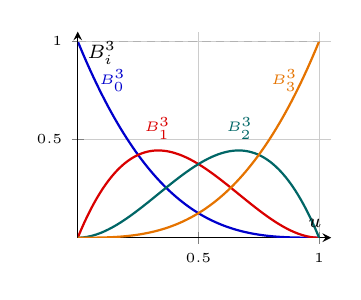
\begin{tikzpicture}
                \begin{axis}[
                    width=4.8cm,
                    height=4.2cm,
                    axis lines=middle,
                    xlabel={$u$},
                    ylabel={$B_i^3$},
                    label style={font=\scriptsize},
                    tick label style={font=\tiny},
                    xmin=0, xmax=1.05,
                    ymin=0, ymax=1.05,
                    xtick={0, 0.5, 1},
                    ytick={0, 0.5, 1},
                    grid=both,
                    grid style={line width=.1pt, draw=gray!20},
                    major grid style={line width=.2pt, draw=gray!40},
                    domain=0:1,
                    samples=80
                ]
                    \addplot[thick, blue!80!black] { (1 - x)^3 };
                    \node[blue!80!black, font=\tiny, anchor=west] at (axis cs: 0.05, 0.8) {$B_0^3$};

                    \addplot[thick, red!85!black] { 3 * x * (1 - x)^2 };
                    \node[red!85!black, font=\tiny, anchor=south] at (axis cs: 0.33, 0.45) {$B_1^3$};

                    \addplot[thick, teal!80!black] { 3 * x^2 * (1 - x) };
                    \node[teal!80!black, font=\tiny, anchor=south] at (axis cs: 0.67, 0.45) {$B_2^3$};

                    \addplot[thick, orange!90!black] { x^3 };
                    \node[orange!90!black, font=\tiny, anchor=east] at (axis cs: 0.95, 0.8) {$B_3^3$};

                    \addplot[densely dashed, gray!60, thin] coordinates {(0, 1) (1, 1)};
                \end{axis}
            \end{tikzpicture}
            \caption{Base de Bernstein}
            \label{fig:bernstein_deg3}
        \end{subfigure}
        \hfill
        % --- Sous-figure (c) : Courbe finale et enveloppe convexe ---
        \begin{subfigure}[b]{0.31\linewidth}
            \centering
            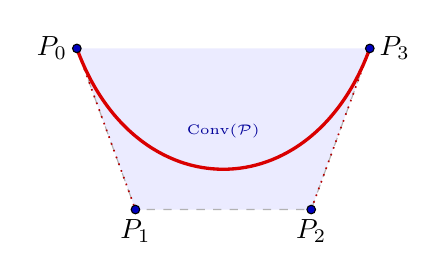
\begin{tikzpicture}[scale=0.62]
                \coordinate (P0) at (0, 3.5);
                \coordinate (P1) at (1.2, 0.2);
                \coordinate (P2) at (4.8, 0.2);
                \coordinate (P3) at (6, 3.5);

                % Enveloppe convexe
                \fill[blue!8] (P0) -- (P1) -- (P2) -- (P3) -- cycle;
                \node[blue!60!black, font=\tiny] at (3, 1.8) {$\mathrm{Conv}(\mathcal{P})$};

                % Polygone et tangentes
                \draw[dashed, gray!60, thin] (P0) -- (P1) -- (P2) -- (P3);
                \draw[dotted, red!70!black, semithick] (P0) -- (P1);
                \draw[dotted, red!70!black, semithick] (P2) -- (P3);

                % Courbe de Bézier
                \draw[very thick, red!85!black] (P0) .. controls (P1) and (P2) .. (P3);

                % Sommets
                \filldraw[fill=blue!75!black, draw=black] (P0) circle (2.5pt) node[left] {$P_0$};
                \filldraw[fill=blue!75!black, draw=black] (P1) circle (2.5pt) node[below] {$P_1$};
                \filldraw[fill=blue!75!black, draw=black] (P2) circle (2.5pt) node[below] {$P_2$};
                \filldraw[fill=blue!75!black, draw=black] (P3) circle (2.5pt) node[right] {$P_3$};
            \end{tikzpicture}
            \caption{Courbe résultante}
            \label{fig:bezier_forme_u}
        \end{subfigure}
        
        \caption{Construction d'une approximation de Bézier cubique : du polygône de contrôle au tracé final borné par l'enveloppe convexe.}
        \label{fig:construction_bezier}
    \end{figure}
\end{example}

\begin{remark}
    En fonction du nombre de points de contrôle, la courbe obtenue aura différentes propriétés : 
    \begin{itemize}
        \item Segment Linéaire : 2 points de contrôle, 
        \item Parabole quardatique : 3 points de contrôle, 
        \item Parabole cubique : 4 points de contrôle. 
    \end{itemize}
\end{remark}

Après plusieurs tracés, on identifie rapidement plusieurs limitations à l'utilisation des courbes de Bézier pour tracer des formes plus complexes. La première est un phénomène d'écrasement lorsque l'on dépasse 5 à 6 points de contrôles. En effet, par définition, la famille des polynômes de Bernstein à utiliser doit sommer à 1, ils doivent donc mécaniquement s'applitir pour respecter cette conrtainte (visible dans la Figure~\ref{fig:bernstein_base_deg7}). Cela produit donc une courbe paramétrique plus applatie (voir Figure~\ref{fig:bezier_aplatissement_deg7}). 

\begin{figure}[htbp]
    \centering
    % --- Sous-figure (a) : Les 8 polynômes de Bernstein de degré 7 ---
    \begin{subfigure}[b]{0.48\textwidth}
        \centering
        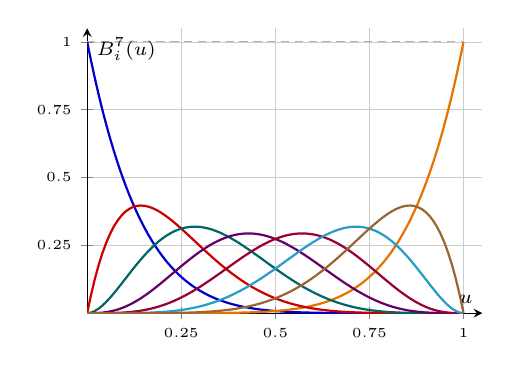
\begin{tikzpicture}
            \begin{axis}[
                width=6.6cm,
                height=5.2cm,
                axis lines=middle,
                xlabel={$u$},
                ylabel={$B_i^7(u)$},
                label style={font=\scriptsize},
                tick label style={font=\tiny},
                xmin=0, xmax=1.05,
                ymin=0, ymax=1.05,
                xtick={0, 0.25, 0.5, 0.75, 1},
                ytick={0, 0.25, 0.5, 0.75, 1},
                grid=both,
                grid style={line width=.1pt, draw=gray!20},
                major grid style={line width=.2pt, draw=gray!40},
                domain=0:1,
                samples=100
            ]
                % B_0^7 et B_7^7 (bords)
                \addplot[thick, blue!80!black] { (1 - x)^7 };
                \addplot[thick, orange!90!black] { x^7 };

                % B_1^7 à B_6^7 (intermédiaires)
                \addplot[thick, red!80!black] { 7 * x * (1 - x)^6 };
                \addplot[thick, teal!80!black] { 21 * x^2 * (1 - x)^5 };
                \addplot[thick, violet!80!black] { 35 * x^3 * (1 - x)^4 };
                \addplot[thick, purple!80!black] { 35 * x^4 * (1 - x)^3 };
                \addplot[thick, cyan!80!black] { 21 * x^5 * (1 - x)^2 };
                \addplot[thick, brown!80!black] { 7 * x^6 * (1 - x) };

                % Ligne de repère de la partition de l'unité
                \addplot[densely dashed, gray!60, thin] coordinates {(0, 1) (1, 1)};
            \end{axis}
        \end{tikzpicture}
        \caption{Base de Bernstein de degré 7 ($B_0^7, \dots, B_7^7$)}
        \label{fig:bernstein_base_deg7}
    \end{subfigure}
    \hfill
    % --- Sous-figure (b) : Courbe aplatie sur 8 sommets ---
    \begin{subfigure}[b]{0.48\textwidth}
        \centering
        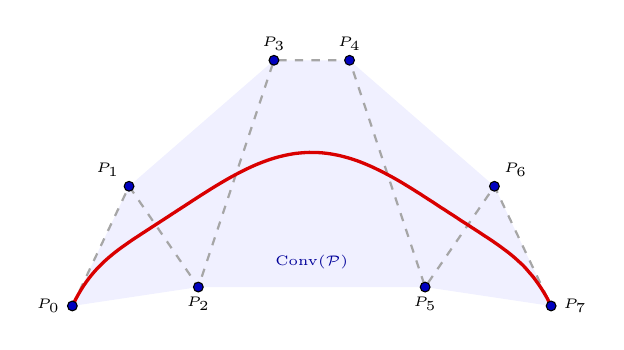
\begin{tikzpicture}[scale=0.8]
            % Coordonnées des 8 sommets (P0 à P7)
            \coordinate (P0) at (0.0, 0.5);
            \coordinate (P1) at (0.9, 2.4);
            \coordinate (P2) at (2.0, 0.8);
            \coordinate (P3) at (3.2, 4.4);
            \coordinate (P4) at (4.4, 4.4);
            \coordinate (P5) at (5.6, 0.8);
            \coordinate (P6) at (6.7, 2.4);
            \coordinate (P7) at (7.6, 0.5);

            % Enveloppe convexe
            \fill[blue!6] (P0) -- (P1) -- (P3) -- (P4) -- (P6) -- (P7) -- (P5) -- (P2) -- cycle;
            \node[blue!60!black, font=\tiny] at (3.8, 1.2) {$\mathrm{Conv}(\mathcal{P})$};

            % Polygone de contrôle
            \draw[dashed, gray!70, thick] (P0) -- (P1) -- (P2) -- (P3) -- (P4) -- (P5) -- (P6) -- (P7);

            % Courbe de Bézier paramétrique de degré 7
            \draw[very thick, red!85!black, domain=0:1, samples=120, smooth]
                plot (
                    {
                        (1-\x)^7 * 0.0 +
                        7*\x*(1-\x)^6 * 0.9 +
                        21*\x^2*(1-\x)^5 * 2.0 +
                        35*\x^3*(1-\x)^4 * 3.2 +
                        35*\x^4*(1-\x)^3 * 4.4 +
                        21*\x^5*(1-\x)^2 * 5.6 +
                        7*\x^6*(1-\x) * 6.7 +
                        \x^7 * 7.6
                    },
                    {
                        (1-\x)^7 * 0.5 +
                        7*\x*(1-\x)^6 * 2.4 +
                        21*\x^2*(1-\x)^5 * 0.8 +
                        35*\x^3*(1-\x)^4 * 4.4 +
                        35*\x^4*(1-\x)^3 * 4.4 +
                        21*\x^5*(1-\x)^2 * 0.8 +
                        7*\x^6*(1-\x) * 2.4 +
                        \x^7 * 0.5
                    }
                );

            % Sommets du polygone
            \filldraw[fill=blue!75!black, draw=black] (P0) circle (2.2pt) node[left=1pt, font=\tiny] {$P_0$};
            \filldraw[fill=blue!75!black, draw=black] (P1) circle (2.2pt) node[above left, font=\tiny] {$P_1$};
            \filldraw[fill=blue!75!black, draw=black] (P2) circle (2.2pt) node[below, font=\tiny] {$P_2$};
            \filldraw[fill=blue!75!black, draw=black] (P3) circle (2.2pt) node[above, font=\tiny] {$P_3$};
            \filldraw[fill=blue!75!black, draw=black] (P4) circle (2.2pt) node[above, font=\tiny] {$P_4$};
            \filldraw[fill=blue!75!black, draw=black] (P5) circle (2.2pt) node[below, font=\tiny] {$P_5$};
            \filldraw[fill=blue!75!black, draw=black] (P6) circle (2.2pt) node[above right, font=\tiny] {$P_6$};
            \filldraw[fill=blue!75!black, draw=black] (P7) circle (2.2pt) node[right=1pt, font=\tiny] {$P_7$};
        \end{tikzpicture}
        \caption{Aplatissement de la courbe paramétrique}
        \label{fig:bezier_courbe_aplatie_deg7}
    \end{subfigure}

    \caption{Phénomène d'aplatissement pour un degré élevé ($n=7$) : l'écrasement des polynômes intermédiaires limite la portée locale des points de contrôle centraux.}
    \label{fig:bezier_aplatissement_deg7}
\end{figure}

% ----------------------------------------------------------------------
\subsection{B-Splines et Vecteur Nodal}

Les B-Splines permettent de pallier le principal défaut des courbes de Bézier (l'absence de contrôle local et l'aplatissement) en découplant le degré polynomial du nombre de points de contrôle.

\begin{definition}[Vecteur nodal et fonctions de base de Cox-de Boor]
    Soit $k \in \N^*$ l'\emph{ordre} de la B-Spline (correspondant à un degré polynomial $p = k - 1$).
    Soit $U = (u_0, u_1, \dots, u_m)$ une suite finie non décroissante de réels appelée \emph{vecteur nodal}.
    
    Pour tout $i \in \llbracket 0, m-k \rrbracket$, les fonctions de base $N_i^k$ sont définies par la récurrence de \emph{Cox-de Boor} :
    \begin{itemize}
        \item \textbf{Initialisation (ordre $1$, degré $0$) :}
        \begin{equation}
            N_i^1(u) = 
            \begin{cases}
                1 & \text{si } u \in [u_i, u_{i+1}[ \\
                0 & \text{sinon}
            \end{cases}
        \end{equation}
        \item \textbf{Hérédité (ordre $k \geqslant 2$, degré $k - 1$) :}
        \begin{equation}
            N_i^k(u) = \frac{u - u_i}{u_{i+k-1} - u_i} N_i^{k-1}(u) + \frac{u_{i+k} - u}{u_{i+k} - u_{i+1}} N_{i+1}^{k-1}(u)
        \end{equation}
    \end{itemize}
    Dans le cas où deux nœuds consécutifs sont confondus, on applique par convention $0/0 = 0$.
\end{definition}

\begin{definition}[Courbe B-Spline]
    Soit une famille de $n+1$ points de contrôle $(P_0, \dots, P_n)$ et un ordre $k$. Le vecteur nodal associé doit nécessairement comporter $m + 1 = n + k + 1$ nœuds.
    
    La \emph{courbe B-Spline} associée est définie sur l'intervalle valide $[u_{k-1}, u_{n+1}]$ par :
    \begin{equation}
        \forall u \in [u_{k-1}, u_{n+1}], \quad P(u) = \sum_{i=0}^n N_i^k(u) P_i
    \end{equation}
    Sur cet intervalle, la partition de l'unité $\sum_{i=0}^n N_i^k(u) = 1$ est vérifiée, garantissant le confinement dans l'enveloppe convexe locale.
\end{definition}

\begin{example}[Degré 1 — Ordre $k=2$]
    Soient $n + 1 = 6$ points de contrôle $(P_0, \dots, P_5)$. On construit la B-Spline de degré $1$ (ordre $k=2$).
    
    Le vecteur nodal uniforme nécessite $m + 1 = (n + 1) + k = 6 + 2 = 8$ nœuds : $U = (0, 1, 2, 3, 4, 5, 6, 7)$. Les fonctions de base $N_i^2(u)$ sont linéaires par morceaux (« dents de scie ») à support compact sur $[u_i, u_{i+2}]$ (Figure~\ref{fig:bspline_deg1_base}).
    La courbe résultante $P(u) = \sum_{i=0}^5 N_i^2(u) P_i$ est définie sur $[u_1, u_6] = [1, 6]$ et réalise l'interpolation linéaire directe des sommets (Figure~\ref{fig:bspline_deg1_vague}).

    \begin{figure}[htbp]
        \centering
        % --- Sous-figure (a) : Les fonctions de base chapeau / dents de scie ---
        \begin{subfigure}[b]{0.48\textwidth}
            \centering
            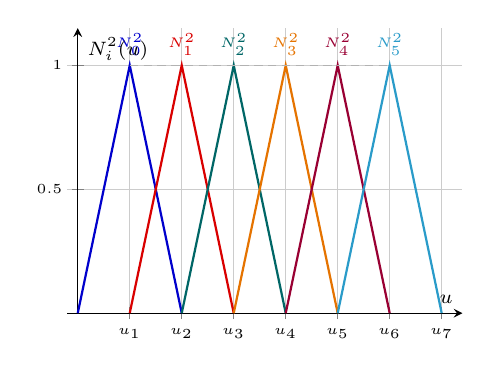
\begin{tikzpicture}
                \begin{axis}[
                    width=6.6cm,
                    height=5.2cm,
                    axis lines=middle,
                    xlabel={$u$},
                    ylabel={$N_i^2(u)$},
                    label style={font=\scriptsize},
                    tick label style={font=\tiny},
                    xmin=-0.2, xmax=7.4,
                    ymin=0, ymax=1.15,
                    xtick={0, 1, 2, 3, 4, 5, 6, 7},
                    xticklabels={$u_0$, $u_1$, $u_2$, $u_3$, $u_4$, $u_5$, $u_6$, $u_7$},
                    ytick={0, 0.5, 1},
                    grid=both,
                    grid style={line width=.1pt, draw=gray!20},
                    major grid style={line width=.2pt, draw=gray!40}
                ]
                    % N_0^2 sur [0, 2]
                    \addplot[thick, blue!80!black] coordinates {(0, 0) (1, 1) (2, 0)};
                    \node[blue!80!black, font=\tiny, above] at (axis cs: 1, 1) {$N_0^2$};

                    % N_1^2 sur [1, 3]
                    \addplot[thick, red!85!black] coordinates {(1, 0) (2, 1) (3, 0)};
                    \node[red!85!black, font=\tiny, above] at (axis cs: 2, 1) {$N_1^2$};

                    % N_2^2 sur [2, 4]
                    \addplot[thick, teal!80!black] coordinates {(2, 0) (3, 1) (4, 0)};
                    \node[teal!80!black, font=\tiny, above] at (axis cs: 3, 1) {$N_2^2$};

                    % N_3^2 sur [3, 5]
                    \addplot[thick, orange!90!black] coordinates {(3, 0) (4, 1) (5, 0)};
                    \node[orange!90!black, font=\tiny, above] at (axis cs: 4, 1) {$N_3^2$};

                    % N_4^2 sur [4, 6]
                    \addplot[thick, purple!80!black] coordinates {(4, 0) (5, 1) (6, 0)};
                    \node[purple!80!black, font=\tiny, above] at (axis cs: 5, 1) {$N_4^2$};

                    % N_5^2 sur [5, 7]
                    \addplot[thick, cyan!80!black] coordinates {(5, 0) (6, 1) (7, 0)};
                    \node[cyan!80!black, font=\tiny, above] at (axis cs: 6, 1) {$N_5^2$};

                    % Ligne de partition de l'unité sum = 1
                    \addplot[densely dashed, gray!60, thin] coordinates {(1, 1) (6, 1)};
                \end{axis}
            \end{tikzpicture}
            \caption{Fonctions de base $N_i^2(u)$ en dents de scie}
            \label{fig:bspline_deg1_base}
        \end{subfigure}
        \hfill
        % --- Sous-figure (b) : Courbe résultante (interpolation linéaire en vague) ---
        \begin{subfigure}[b]{0.48\textwidth}
            \centering
            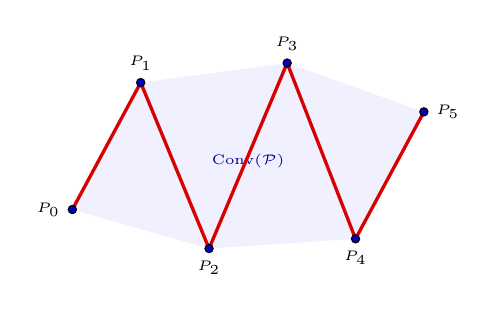
\begin{tikzpicture}[scale=0.62]
                % Coordonnées des 6 sommets formant une onde / vague
                \coordinate (P0) at (0.0, 1.2);
                \coordinate (P1) at (1.4, 3.8); % crête 1
                \coordinate (P2) at (2.8, 0.4); % creux 1
                \coordinate (P3) at (4.4, 4.2); % crête 2
                \coordinate (P4) at (5.8, 0.6); % creux 2
                \coordinate (P5) at (7.2, 3.2);

                % Enveloppe convexe locale / globale
                \fill[blue!6] (P0) -- (P1) -- (P3) -- (P5) -- (P4) -- (P2) -- cycle;
                \node[blue!60!black, font=\tiny] at (3.6, 2.2) {$\mathrm{Conv}(\mathcal{P})$};

                % Polygone de contrôle en pointillés
                \draw[dashed, gray!70, thick] (P0) -- (P1) -- (P2) -- (P3) -- (P4) -- (P5);

                % Courbe B-Spline de degré 1 (interpolation linéaire exacte entre les points)
                \draw[very thick, red!85!black] (P0) -- (P1) -- (P2) -- (P3) -- (P4) -- (P5);

                % Points de contrôle
                \filldraw[fill=blue!75!black, draw=black] (P0) circle (2.4pt) node[left=1pt, font=\tiny] {$P_0$};
                \filldraw[fill=blue!75!black, draw=black] (P1) circle (2.4pt) node[above=1pt, font=\tiny] {$P_1$};
                \filldraw[fill=blue!75!black, draw=black] (P2) circle (2.4pt) node[below=1pt, font=\tiny] {$P_2$};
                \filldraw[fill=blue!75!black, draw=black] (P3) circle (2.4pt) node[above=1pt, font=\tiny] {$P_3$};
                \filldraw[fill=blue!75!black, draw=black] (P4) circle (2.4pt) node[below=1pt, font=\tiny] {$P_4$};
                \filldraw[fill=blue!75!black, draw=black] (P5) circle (2.4pt) node[right=1pt, font=\tiny] {$P_5$};
            \end{tikzpicture}
            \caption{Trajectoire linéaire par morceaux}
            \label{fig:bspline_deg1_vague}
        \end{subfigure}

        \caption{B-Spline de degré 1 sur 6 points de contrôle : support compact à deux intervalles $[u_i, u_{i+2}]$ et interpolation linéaire continue $C^0$ épousant le profil en vague sans aplatissement.}
        \label{fig:bspline_deg1_complet}
    \end{figure}
\end{example}

\begin{example}[Degré 2 — Ordre $k=3$]
    En conservant les $6$ mêmes points de contrôle, on choisit cette fois un degré $2$ (ordre $k=3$).
    
    Le vecteur nodal requiert désormais $m + 1 = 6 + 3 = 9$ nœuds : $U = (0, 1, 2, 3, 4, 5, 6, 7, 8)$. Les fonctions de base $N_i^3(u)$ sont quadratiques par morceaux de classe $\mathcal{C}^1$ sur $[u_i, u_{i+3}]$ (Figure~\ref{fig:bspline_deg2_base}).
    La courbe $P(u) = \sum_{i=0}^5 N_i^3(u) P_i$ est évaluée sur $[u_2, u_6] = [2, 6]$ et produit une trajectoire lissée sans angle vif (Figure~\ref{fig:bspline_deg2_vague}).

    \begin{figure}[htbp]
        \centering
        % --- Sous-figure (a) : Fonctions de base quadratiques C1 ---
        \begin{subfigure}[b]{0.48\textwidth}
            \centering
            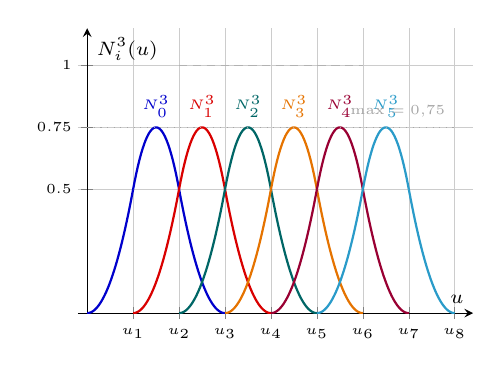
\begin{tikzpicture}
                \begin{axis}[
                    width=6.6cm,
                    height=5.2cm,
                    axis lines=middle,
                    xlabel={$u$},
                    ylabel={$N_i^3(u)$},
                    label style={font=\scriptsize},
                    tick label style={font=\tiny},
                    xmin=-0.2, xmax=8.4,
                    ymin=0, ymax=1.15,
                    xtick={0, 1, 2, 3, 4, 5, 6, 7, 8},
                    xticklabels={$u_0$, $u_1$, $u_2$, $u_3$, $u_4$, $u_5$, $u_6$, $u_7$, $u_8$},
                    ytick={0, 0.5, 0.75, 1},
                    grid=both,
                    grid style={line width=.1pt, draw=gray!20},
                    major grid style={line width=.2pt, draw=gray!40}
                ]
                    % Fonction de base type de degré 2 sur [0, 3] décalée :
                    % N(t) = 0.5*t^2 sur [0,1], 0.75 - (t-1.5)^2 sur [1,2], 0.5*(3-t)^2 sur [2,3]
                    \addplot[thick, blue!80!black, domain=0:1, samples=30] {0.5*x^2};
                    \addplot[thick, blue!80!black, domain=1:2, samples=30] {0.75 - (x-1.5)^2};
                    \addplot[thick, blue!80!black, domain=2:3, samples=30] {0.5*(3-x)^2};
                    \node[blue!80!black, font=\tiny, above] at (axis cs: 1.5, 0.75) {$N_0^3$};

                    \addplot[thick, red!85!black, domain=1:2, samples=30] {0.5*(x-1)^2};
                    \addplot[thick, red!85!black, domain=2:3, samples=30] {0.75 - (x-2.5)^2};
                    \addplot[thick, red!85!black, domain=3:4, samples=30] {0.5*(4-x)^2};
                    \node[red!85!black, font=\tiny, above] at (axis cs: 2.5, 0.75) {$N_1^3$};

                    \addplot[thick, teal!80!black, domain=2:3, samples=30] {0.5*(x-2)^2};
                    \addplot[thick, teal!80!black, domain=3:4, samples=30] {0.75 - (x-3.5)^2};
                    \addplot[thick, teal!80!black, domain=4:5, samples=30] {0.5*(5-x)^2};
                    \node[teal!80!black, font=\tiny, above] at (axis cs: 3.5, 0.75) {$N_2^3$};

                    \addplot[thick, orange!90!black, domain=3:4, samples=30] {0.5*(x-3)^2};
                    \addplot[thick, orange!90!black, domain=4:5, samples=30] {0.75 - (x-4.5)^2};
                    \addplot[thick, orange!90!black, domain=5:6, samples=30] {0.5*(6-x)^2};
                    \node[orange!90!black, font=\tiny, above] at (axis cs: 4.5, 0.75) {$N_3^3$};

                    \addplot[thick, purple!80!black, domain=4:5, samples=30] {0.5*(x-4)^2};
                    \addplot[thick, purple!80!black, domain=5:6, samples=30] {0.75 - (x-5.5)^2};
                    \addplot[thick, purple!80!black, domain=6:7, samples=30] {0.5*(7-x)^2};
                    \node[purple!80!black, font=\tiny, above] at (axis cs: 5.5, 0.75) {$N_4^3$};

                    \addplot[thick, cyan!80!black, domain=5:6, samples=30] {0.5*(x-5)^2};
                    \addplot[thick, cyan!80!black, domain=6:7, samples=30] {0.75 - (x-6.5)^2};
                    \addplot[thick, cyan!80!black, domain=7:8, samples=30] {0.5*(8-x)^2};
                    \node[cyan!80!black, font=\tiny, above] at (axis cs: 6.5, 0.75) {$N_5^3$};

                    % Repère de la partition de l'unité sum = 1 sur le domaine valide [2, 6]
                    \addplot[densely dashed, gray!60, thin] coordinates {(2, 1) (6, 1)};
                    \addplot[dotted, gray!70, thin] coordinates {(0, 0.75) (8, 0.75)};
                    \node[gray!70, font=\tiny, anchor=south east] at (axis cs: 8, 0.75) {$\max = 0{,}75$};
                \end{axis}
            \end{tikzpicture}
            \caption{Fonctions de base $N_i^3(u)$ de degré 2 ($\mathcal{C}^1$)}
            \label{fig:bspline_deg2_base}
        \end{subfigure}
        \hfill
        % --- Sous-figure (b) : Courbe résultante lissée ---
        \begin{subfigure}[b]{0.48\textwidth}
            \centering
            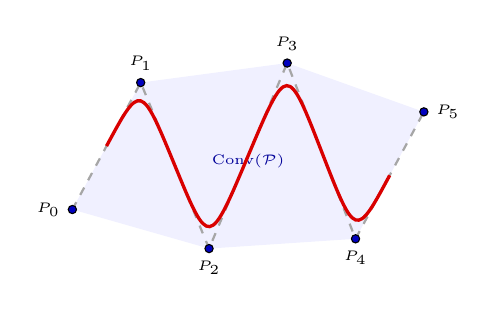
\begin{tikzpicture}[scale=0.62]
                % Mêmes 6 sommets formant l'onde
                \coordinate (P0) at (0.0, 1.2);
                \coordinate (P1) at (1.4, 3.8);
                \coordinate (P2) at (2.8, 0.4);
                \coordinate (P3) at (4.4, 4.2);
                \coordinate (P4) at (5.8, 0.6);
                \coordinate (P5) at (7.2, 3.2);

                % Enveloppe convexe
                \fill[blue!6] (P0) -- (P1) -- (P3) -- (P5) -- (P4) -- (P2) -- cycle;
                \node[blue!60!black, font=\tiny] at (3.6, 2.2) {$\mathrm{Conv}(\mathcal{P})$};

                % Polygone de contrôle
                \draw[dashed, gray!70, thick] (P0) -- (P1) -- (P2) -- (P3) -- (P4) -- (P5);

                % Trajectoire B-Spline de degré 2 (raccord parabolique C1 par morceaux)
                % Les milieux des segments servent de points de contact/raccord
                \coordinate (M01) at (0.7, 2.5);
                \coordinate (M12) at (2.1, 2.1);
                \coordinate (M23) at (3.6, 2.3);
                \coordinate (M34) at (5.1, 2.4);
                \coordinate (M45) at (6.5, 1.9);

                \draw[very thick, red!85!black] 
                    (M01) .. controls (P1) .. (M12)
                          .. controls (P2) .. (M23)
                          .. controls (P3) .. (M34)
                          .. controls (P4) .. (M45);

                % Points de contrôle
                \filldraw[fill=blue!75!black, draw=black] (P0) circle (2.4pt) node[left=1pt, font=\tiny] {$P_0$};
                \filldraw[fill=blue!75!black, draw=black] (P1) circle (2.4pt) node[above=1pt, font=\tiny] {$P_1$};
                \filldraw[fill=blue!75!black, draw=black] (P2) circle (2.4pt) node[below=1pt, font=\tiny] {$P_2$};
                \filldraw[fill=blue!75!black, draw=black] (P3) circle (2.4pt) node[above=1pt, font=\tiny] {$P_3$};
                \filldraw[fill=blue!75!black, draw=black] (P4) circle (2.4pt) node[below=1pt, font=\tiny] {$P_4$};
                \filldraw[fill=blue!75!black, draw=black] (P5) circle (2.4pt) node[right=1pt, font=\tiny] {$P_5$};
            \end{tikzpicture}
            \caption{Courbe lissée $\mathcal{C}^1$ par morceaux}
            \label{fig:bspline_deg2_vague}
        \end{subfigure}

        \caption{B-Spline uniforme de degré 2 sur 6 points de contrôle.}
        \label{fig:bspline_deg2_complet}
    \end{figure}
\end{example}

% % ----------------------------------------------------------------------
% \subsection{Formes rationnelles et NURBS}

% Bien que les B-Splines polynomiales résolvent le problème du contrôle local et de l'aplatissement, elles souffrent d'une limitation algébrique majeure : l'impossibilité intrinsèque de modéliser exactement les coniques[cite: 1].

% \subsubsection{Limitation des représentations polynomiales sur les coniques}

% En conception assistée par ordinateur (CAO), les primitives géométriques circulaires (cylindres de perçage, congés de raccordement, tores) sont omniprésentes. Or, le résultat suivant montre qu'une courbe polynomiale ne peut pas tracer rigoureusement un cercle.

% \begin{proposition}[Impossibilité du cercle polynomial]
%     Il n'existe aucun couple de polynômes réels non constants $(x, y) \in \R[X]^2$ tel que la courbe paramétrée $u \mapsto (x(u), y(u))$ trace un arc de cercle non trivial.
% \end{proposition}

% \begin{proof}
%     Supposons qu'il existe deux polynômes $x, y \in \R[X]$ et un intervalle non trivial $I \subset \R$ vérifiant l'équation implicite du cercle unité :
%     \begin{equation}
%         \forall u \in I, \quad x(u)^2 + y(u)^2 = 1.
%     \end{equation}
%     Considérons le polynôme $Q(X) = x(X)^2 + y(X)^2 - 1 \in \R[X]$. L'ensemble de ses racines contient $I$. Comme un intervalle réel non vide contient une infinité de points et qu'un polynôme non nul n'admet qu'un nombre fini de racines (majoré par son degré), $Q$ est nécessairement le polynôme nul dans $\R[X]$. On en déduit l'identité formelle :
%     \begin{equation}
%         x(X)^2 + y(X)^2 = 1 \quad \text{dans } \R[X].
%     \end{equation}
%     Supposons maintenant que la courbe ne soit pas stationnaire, c'est-à-dire que $\deg(x) \ge 1$ ou $\deg(y) \ge 1$. Notons $d = \max(\deg(x), \deg(y)) \ge 1$.
%     Les monômes de plus haut degré de $x$ et $y$ s'écrivent respectivement $a X^d$ et $b X^d$ avec $(a, b) \in \R^2 \setminus \{(0, 0)\}$.
%     Dans la somme $x(X)^2 + y(X)^2$, le coefficient devant le monôme $X^{2d}$ vaut :
%     \begin{equation}
%         a^2 + b^2 > 0.
%     \end{equation}
%     Puisque les coefficients sont réels, aucune compensation n'est possible à l'ordre maximal. On en déduit :
%     \begin{equation}
%         \deg\big(x(X)^2 + y(X)^2\big) = 2d \ge 2.
%     \end{equation}
%     Or, $\deg(1) = 0$, ce qui conduit à une contradiction directe ($2d = 0$). Ainsi, les seuls polynômes vérifiant cette relation sont constants : aucun arc continu de cercle ne peut être tracé de façon purement polynomiale.
% \end{proof}

% \subsubsection{Définition des NURBS}

% Pour contourner ce verrou, on passe à des \emph{fractions rationnelles} en autorisant un dénominateur commun $W(u)$ :
% \begin{equation}
%     x(u) = \frac{X(u)}{W(u)}, \quad y(u) = \frac{Y(u)}{W(u)}.
% \end{equation}
% L'équation du cercle unité devient alors une identité pythagoricienne dans $\R[X]$ :
% \begin{equation}
%     X(u)^2 + Y(u)^2 = W(u)^2,
% \end{equation}
% qui admet des solutions polynomiales non triviales de degré 2 (liées aux formules classiques en $t = \tan(\theta/2)$ : $X(u) = 1 - u^2$, $Y(u) = 2u$ et $W(u) = 1 + u^2$).

% Cette formulation conduit naturellement aux \emph{NURBS} (\emph{Non-Uniform Rational B-Splines})[cite: 1].

% \begin{definition}[Courbe NURBS]
%     Soit une famille de $n+1$ points de contrôle $(P_0, \dots, P_n) \in \mathcal{E}^{n+1}$, un vecteur nodal $U$ et des fonctions de base B-Splines $N_i^k(u)$ d'ordre $k$ associées[cite: 1]. On associe à chaque point de contrôle un \emph{poids} scalaire strictement positif $w_i > 0$[cite: 1].
    
%     La \emph{courbe NURBS} associée est l'application paramétrique définie par :
%     \begin{equation}
%         \boxed{P(u) = \frac{\sum_{i=0}^n w_i N_i^k(u) P_i}{\sum_{i=0}^n w_i N_i^k(u)} = \sum_{i=0}^n R_i^k(u) P_i}
%     \end{equation}
%     où les fonctions de base rationnelles $R_i^k$ sont données par[cite: 1] :
%     \begin{equation}
%         R_i^k(u) = \frac{w_i N_i^k(u)}{\sum_{j=0}^n w_j N_j^k(u)}.
%     \end{equation}
% \end{definition}

% \begin{proposition}[Propriétés des NURBS]
%     Les fonctions rationnelles $R_i^k$ et la courbe NURBS satisfont :
%     \begin{enumerate}
%         \item \textbf{Partition de l'unité et positivité :} pour tout $u$ sur le domaine valide, $\sum_{i=0}^n R_i^k(u) = 1$ et $R_i^k(u) \ge 0$, garantissant le confinement strict dans l'enveloppe convexe locale des points de contrôle.
%         \item \textbf{Généralisation des B-Splines :} si tous les poids sont égaux ($w_i = w > 0$), les termes se simplifient et on retrouve la B-Spline polynomiale classique.
%         \item \textbf{Représentation exacte des coniques :} le choix adéquat de poids permet de tracer rigoureusement des cercles, ellipses et hyperboles avec un degré polynomial minimal ($k=3$, degré 2)[cite: 1].
%         \item \textbf{Invariance projective :} les NURBS sont invariantes par projection perspective (essentiel pour le rendu graphique sur écran), propriété que ne possèdent pas les B-Splines polynomiales.
%     \end{enumerate}
% \end{proposition}